
\section{External Models}

Many external models are used in simulation to accurately depict the
environment. The paper here begins with the Earth Magnetic Field
and Gravitational Models. The magnetic field model comes from the Geographic
Library model which uses the EMM2015 magnetic field model. The
gravitational model comes from the EGM2008 model
\cite{GeographicLib}.

\subsection{GPS Coordinates to Cartesian Coordinates}

All external models below imply a spherical world with an Earth Centered Inertial (ECI) frame at the center of the planet. However, often times for small UAV applications it is useful to convert the GPS coordinates (latitude, longitude, altitude, $(\lambda_{LAT},\lambda_{LON},h)$) to a flat earth approximation where the x-axis is pointing North, the y-axis is pointing east and the z-axis is pointing towards the center of the planet. This is similar to spherical coordinates which is explained later on but in this case the axis system is cartesian rather than spherical. This is useful in obtaining the position of the vehicle which can be used to approximate heading and speed which again is explained in another section. The equations to convert LLH (latitude,longitude, altitude) to a cartesian coordinate system are given below. Note that these equations assume that the vehicle creates an origin point to define as the center of the inertial frame which is on the surface of the planet rather than the center of the planet $\lambda_{LAT,0},\lambda_{LON,0}$. Typically when the vehicle gets its first valid GPS coordinate, that point is set as the origin.
\begin{equation}
\begin{matrix}
x = \kappa (\lambda_{LAT} - \lambda_{LAT,0}) \\
y = \kappa (\lambda_{LON} - \lambda_{LON,0}) cos(\frac{\pi}{180}\lambda_{LAT,0}) \\
z = -h
\end{matrix}
\end{equation}
In the equation above $\kappa = 60.0*(Feet/NauticalMiles)*(Meters/Feet)$ which essentially converts degrees from the LLH coordinates first to nautical miles and then to feet and then to meters. For example, if the vehicle moves North 1 degree that is equivalent to 60 nautical miles on the surface. Vice versa, 1 nautical mile on the surface is equal to one minute or a 60th of a degree in latitude. The conversion from nautical miles to feet is 6076.11548556 and feet to meters is 0.3048. Note that often time is is good to convert the cartesian coordinates back to LLH coordinates. That inversion is shown below.
\begin{equation}
\lambda_{LAT} = \frac{x}{\kappa} + \lambda_{LAT,0}
\end{equation}
\begin{equation}
\lambda_{LON} = \frac{y}{\kappa cos(\lambda_{LAT,0} \frac{\pi}{180})} + \lambda_{LON,0}\\
\end{equation}
\begin{equation}
h = -z
\end{equation}

\subsection{Density Model}

The density model is simply given as an exponential model. 
\begin{equation}
     \rho = \rho_s e^{-\sigma h}
\end{equation}
where $\rho_s$ is the density at sea-level, $h$ is the altitude above
the Earth in kilometers and $\sigma = 0.1354 km^{-1}$ is known as the
scale height \cite{Jacchia1,Jacchia2,Jacchia3}.  

\subsection{Magnetic Field Model}\label{s:magnetic_field}

The Magnetic Field model used in this simulation stems from the
Enhanced Magnetic Field Model (EMM2015) (\cite{EMM2015}). The Earth's magnetic is a
complex superposition of multiple sources including the inner core and
outer core of the planet. Models have been created that use spherical
harmonics to compute the magnetic field at any location around the
Earth. The EMM2015 model uses a 720 order model increasing the spatial
resolution down to 56 km. This model was compiled from multiple
sources including but not limited to satellite and marine data. It
also includes data from the European Space Agency's Swarm satellite
mission. In order to include this harmonic mesh data into this simulation,
the GeographicLib module written in C++ is included in the
simulation (\cite{GeographicLib}). Note that I take no credit for this
model. This section only serves to explain the model. The result of
utilizing this model is the ability to provide any position coordinate
of the satellite to the module and have
the model return the magnetic field strength in East, North, Vertical
Coordinates. Specifically, the inputs to the model are 
the position $x,y,z$ of the satellite assuming an inertial frame with
the z-axis pointing through the north pole and the x axis pointing
through the equator at the prime meridian as seen in Figure
\ref{f:spherical}. This is known as the Earth-Centered Inertial
(ECI) coordinate system (\cite{ECI}).
\begin{figure}[H]
  \begin{center}
  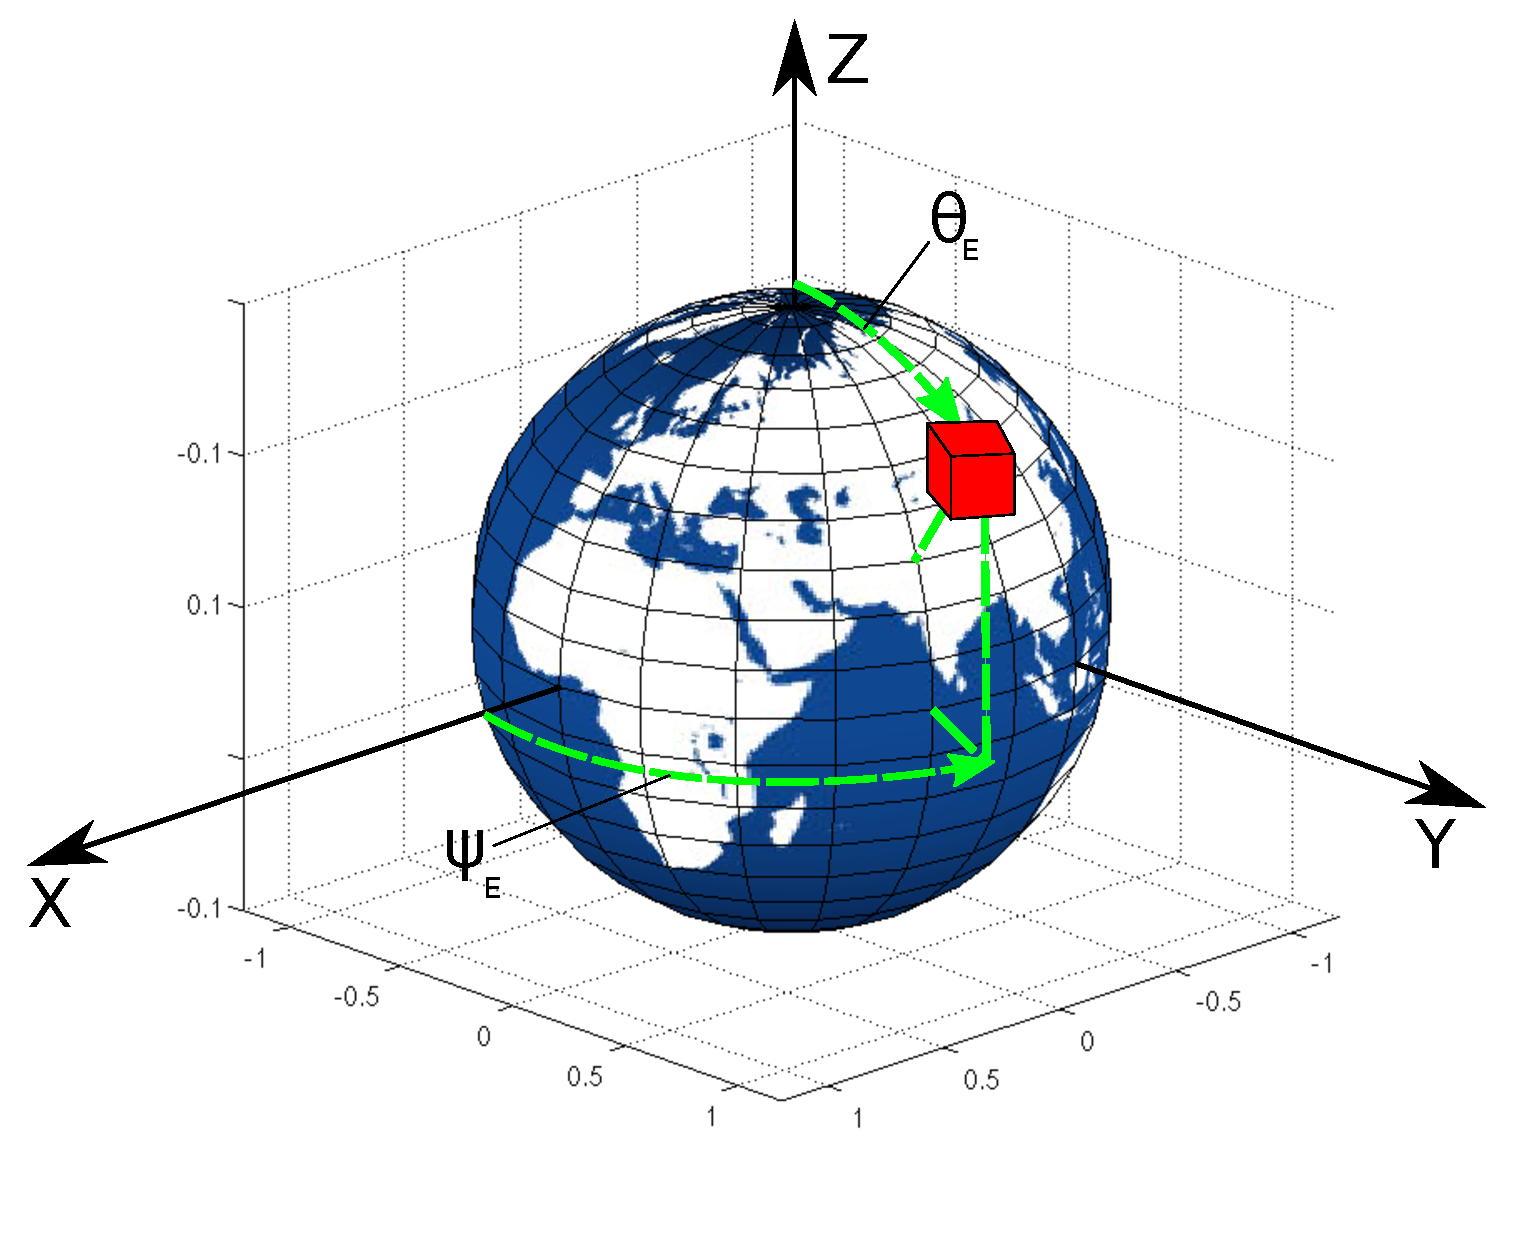
\includegraphics[height=100mm, width=120mm]{Figures/ECI.pdf}
  \end{center}
  \caption{Earth-Centered Inertial Frame and Spherical Coordinate Frame}\label{f:spherical}
\end{figure}
\noindent In order to connect these inertial coordinates ($x,y,z$) to
be used in the EMM2015 model, the latitude, longitude and height above
the surface of the Earth are required. To do this, the coordinates are
converted into spherical coordinates using the equations below.
\begin{equation}\label{e:spherical_coordinates}
  \begin{matrix}
    \rho = \sqrt{x^2+y^2+z^2} \\
    \phi_E = 0 \\
    \theta_E = cos^{-1}\left( \frac{z}{\rho}\right) \\
    \psi_E = tan^{-1}\left( \frac{y}{x}\right)
  \end{matrix}
\end{equation}
Note that $\rho,\phi_E,\theta_E,\psi_E$ are related to latitude and
longitude coordinates but not quite the same. In order to obtain the
latitude and longitude coordinates the following equations are
used. The height is simply the distance from the center of the ECI
frame minus the reference height from the approximation of Earth as an
ellipsoid ($R_{\Earth}=6,371,393~meters$). Note that the angles from Equation
\ref{e:spherical_coordinates} are converted to degrees. 
\begin{equation}
  \begin{matrix}
    \lambda_{LAT} = 90 - \theta_E\frac{180}{\pi}\\
    \lambda_{LON} = \psi_E\frac{180}{\pi} \\
    h = \rho - R_{\Earth}
  \end{matrix}
\end{equation}
The inputs to the EMM2015 model are the latitude, longitude and height. The inverse of the above two equations are given below. These would be used in the event a latitude and longitude coordinate is given and there is a need to obtain the x,y and z coordinates in the ECI frame. The first step is to convert latitude, longitude and altitude and convert that to standard spherical angles and distance from the center of the planet.
\begin{equation}
\begin{matrix}
\theta_E = (90 - \lambda_{LAT})\frac{\pi}{180}\\
\psi_E = \lambda_{LON}\frac{\pi}{180}\\
\rho = h + R_{\Earth}
\end{matrix}
\end{equation}
Once that is complete the extraction of x,y and z are computed by the equation below.
\begin{equation}
\begin{matrix}
x = \rho sin(\theta_E) cos(\psi_E)\\
y = \rho sin(\theta_E) sin(\psi_E)\\
z = \rho cos(\theta_E)
\end{matrix}
\end{equation}
The output from the EMM2015 model is in the East, North, Vertical (ENV) reference frame
where the x-axis is East pointing in the direction of the rotation on
the Earth, the y-axis is North pointing towards the North pole and
finally the z-axis is the Vertical component that is always pointing
radially away from the center of the Earth. In order to get the
coordinates into the ECI frame the coordinates must first me converted
to the North, East, Down reference frame (NED). In this case the
x-axis is pointing North, the y-axis pointing East and the z-axis is
always pointing towards the center of the Earth and called Down. The
equation to rotate from the ENV frame to NED frame is shown below.
\begin{equation}
  \begin{Bmatrix} \beta_x \\ \beta_y \\ \beta_z \end{Bmatrix}_{NED}
  = \begin{bmatrix} 0 & 1 & 0 \\ 1 & 0 & 0 \\ 0 & 0 & -1 \end{bmatrix} \begin{Bmatrix} \beta_x \\ \beta_y \\ \beta_z \end{Bmatrix}_{ENV}
\end{equation}
Once the magnetic field is in the NED reference frame it can then be
rotated to the inertial frame using the following equation where $\vec{\beta}_{NED}$ is the
magnetic field in the NED coordinate system and $\vec{\beta}_I$ is the
magnetic field in the inertial frame. 
\begin{equation}\label{e:sph_inertial}
  \vec{\beta}_I = {\bf T}_{IB}(0,\theta_E+\pi,\psi_E)\vec{\beta}_{NED}
\end{equation}
The matrix ${\bf T}_{IB}(\phi,\theta,\psi)$ represents the transformation
matrix from the spherical reference frame to the inertial reference
frame. Note that there is no rotation about the x-axis through
$\phi_E$ and the pitch rotation is augmented by $\pi$ because of the
switch between North, East, Down (NED) and the z-axis of the ECI
pointing through the North pole. The result of these equations, is the
ability to obtain the magnetic field  
across an entire orbit. Figure \ref{f:orbit} shows an example 56
degree inclination orbit, 600 km above the Earth's surface. The orbit
begins with the satellite above the equator and the prime meridian and
assumes the Earth does not rotate.
\begin{figure}[H]
  \begin{center}
  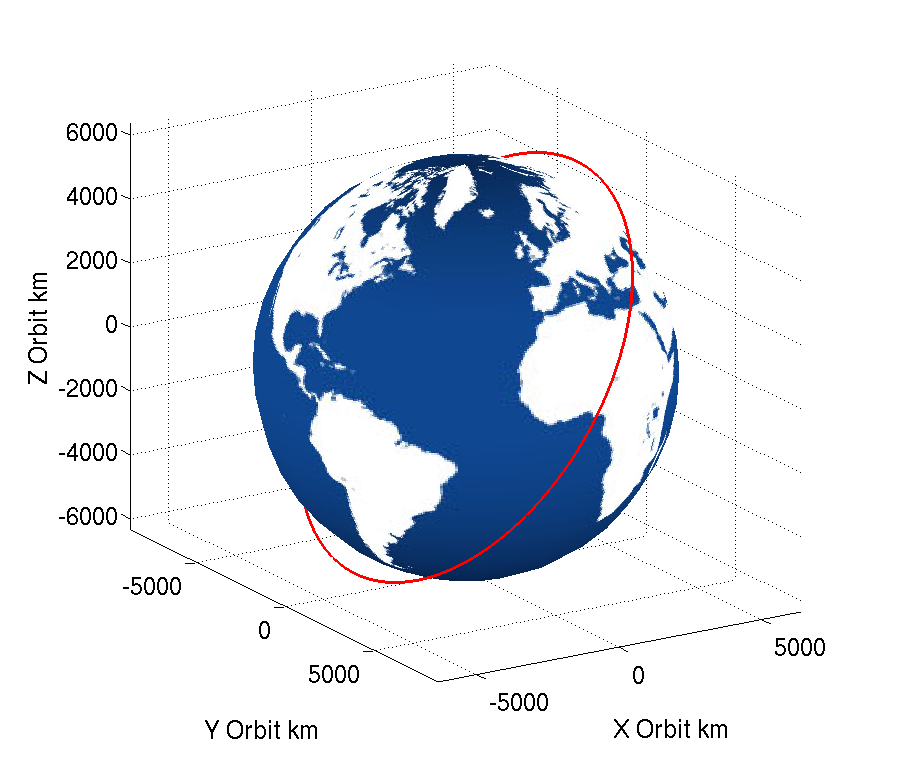
\includegraphics[height=70mm, width=80mm]{Figures/Earth_Orbit.png}
  \end{center}
  \caption{Example 56 Degree Inclination Orbit at 600 km above Earth's
  Surface}\label{f:orbit}
\end{figure}
Figure \ref{f:mag_orbit} shows the magnetic field during the orbit in the
inertial frame. PCI stands for Planet Centered Inertial which in this
case is the same as the ECI frame since the planet is Earth. 
\begin{figure}[H]
  \begin{center}
  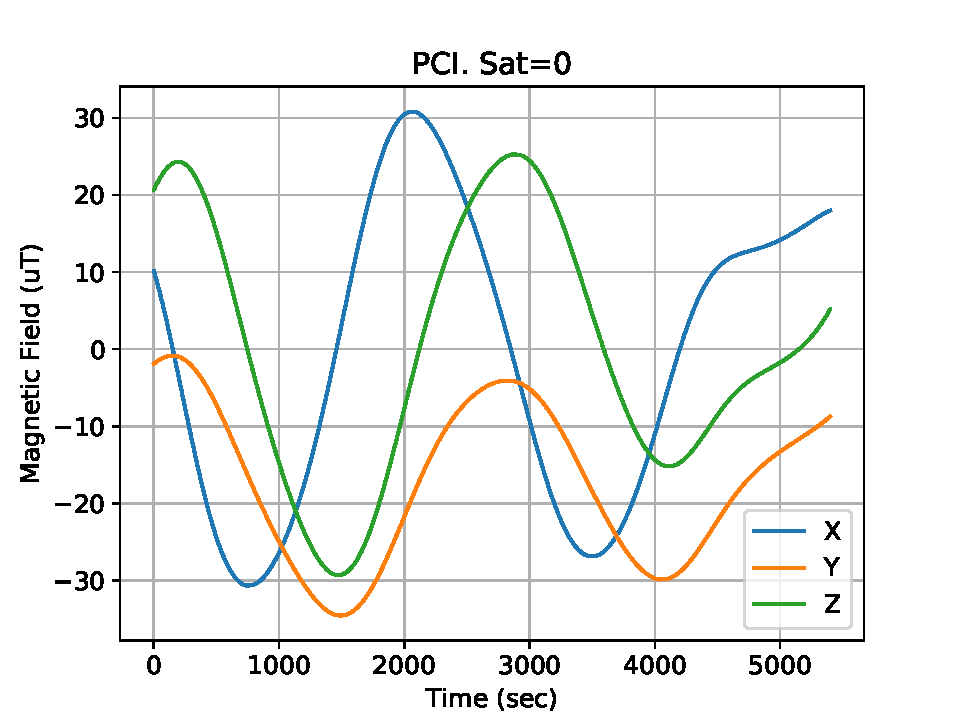
\includegraphics[width=90mm]{Figures/Magnetic_Field_Orbit}
  \end{center}
  \caption{Magnetic Field of Earth in Inertial Frame for 56 Degree
    Orbit at 600 km Above Surface}\label{f:mag_orbit}
\end{figure}
For a satellite in LEO, the spacecraft will experience a magnetic
dipole moment. The magnetic dipole moment is caused by noting that the
structure of the satellite is metal with current that creates its own
magnetic field. The magnetic dipole moment torque is given by
computing the torque produced by the magnetic field of the Earth
interacting with the metallic structure of the satellite. First the
dipole constant $d_s=2.64E-03~N-m/T$ is the assumed value for torque
as a function of Tesla in LEO. This constant is derived by assuming
the torque from this disturbance at 500 km above the surface is the
same as the solar radiation torque. Using this constant, the torque is
given by the equation below where $\vec{\beta}_I$ is the magnetic
field strength of Earth in the inertial frame. The direction of the
torque is assumed to be in the same direction of the magnetic field
since the structure is not fully modeled. Although not accurate, the
goal is to approximate the magnitude as closely as possible.  
\begin{equation}
    \vec{M}_{MD}=\vec{\beta}_I d_s
\end{equation}

\subsection{Gravitational Models}

Three types of gravitational models can be used. The first is the
Newtonian gravitational model that assumes all planets are point
masses with no volume. The result of the gravitational field vector is
then
\begin{equation}
  \vec{F}_{\Earth} = -G\frac{m_{\Earth} m_s}{r^2}\hat{r}
\end{equation}
where $G$ is the gravitational constant, $\Earth$ denotes the planet
applying the gravitational field, $m_\Earth$ is the mass of the
planet, $m_s$ is the mass of the satellite and $\vec{r}$ is a distance
vector from the center of the planet to the satellite. The vector
$\hat{r}$ is just the unit vector of $\vec{r}$ while $r$ is the
magnitude of $\vec{r}$.
\begin{equation}
  \hat{r} = \vec{r}/r
\end{equation}
In component form, $\vec{r} = [x;y;z]^T$. Substituting that component
form into the two equations above results in the component form of the
gravity model which can be better suited for non-vectorized
programming syntax.
\begin{equation}
\begin{Bmatrix}F_{x\Earth}\\F_{y\Earth}\\F_{z\Earth}\end{Bmatrix} = -G\frac{m_{\Earth}
  m_s}{r^3}\begin{Bmatrix}x\\y\\z\end{Bmatrix}
\end{equation}
The second gravitational field model stems from the
Earth Gravity Model (EGM2008) \cite{EGM2008} which can also be found
in the GeographicLib module \cite{GeographicLib}. This model compute's
Earths gravitational field at any point in three dimensional
space. The model takes in coordinates in the ECI frame and returns the
gravitational acceleration in the ECI frame thus no rotation is
required. Just like the EMM2015 model this model uses spherical
harmonics and a reference ellipsoid. The reference ellipsoid is then
updated with gravity disturbances such as non-uniform geoid
heights. This model is an upgrade from EGM84 and EGM96 which only
used models of order 180 and 360 respectively. The EGM2008 model as a
comparison uses a model of order 2190. Figure \ref{f:grav_orbit} shows
the gravitational acceleration vector during a 56 degree orbit at 600 km above the
Earth's surface. The x-axis has been non-dimensionalized to 
represent the entire orbit. Thus when the x-axis is equal to 100 the
satellite has completed one orbit.
\begin{figure}[H]
  \begin{center}
  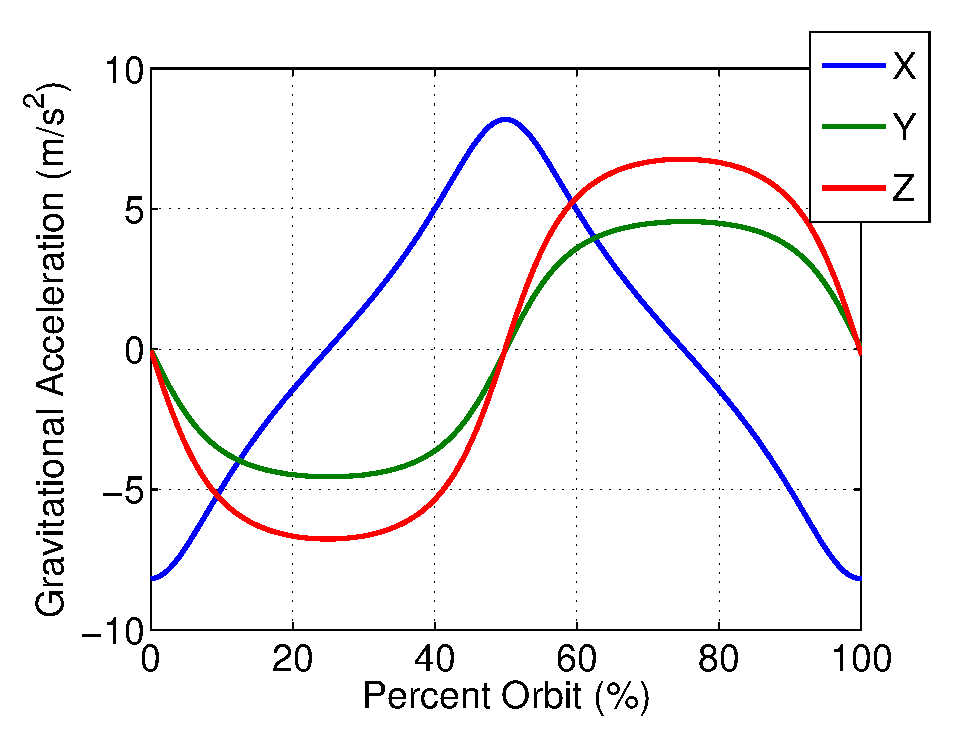
\includegraphics[height=80mm, width=100mm]{Figures/Gravity_Field_Orbit}
  \end{center}
  \caption{Gravitational Field of Earth in Inertial Frame for 56 Degree
    Orbit at 600 km Above Surface}\label{f:grav_orbit}
\end{figure}

For a satellite in LEO, the vehicle will experience a gravity gradient
torque. The gravity gradient torque is given by computing the
gravitational force at one end of the satellite and the other denoted
as $\vec{F}(\vec{r}_B)$ and $\vec{F}(\vec{r}_T)$ for bottom and top
respectively. The torques are then crossed with the distance from the
center of mass to the top of the satellite. It is assumed that the
satellite is symmetric and thus, the torque is just the difference
between the two forces crossed with the vector from the CG to one side
of the satellite. 
\begin{equation}
    \vec{M}_G = {\bf S}(\vec{F}(\vec{r}_B)-\vec{F}(\vec{r}_T))\vec{r}_{CG-B}
\end{equation}

The third gravitational field model assumes the vehicle is close to
the surface such as a quadcopter or aircraft. In this case the
gravitational field is held at a constant and equal to $9.81~m/s^2$.
\begin{equation}\label{e:wforce}
\begin{Bmatrix} X_W \\ Y_W \\ Z_W \end{Bmatrix} = mg \begin{Bmatrix}
-s_{\theta} \\ s_{\phi}c_{\theta} \\ c_{\phi}c_{\theta} \end{Bmatrix}
\end{equation}

\subsection{Earth Orbital Elements}\label{s:ephemeris}

Assuming that the Sun is the central inertial reference point, it is
possible to obtain the position of Earth at any point in time using
well documented orbital elements of the Earth. This formulation
follows the derivation by JPL and can be found at \cite{JPL}. In order
to obtain the position of the Earth, the Julian Day must be
obtained. The Julian Day of January 1st, 2019 is 2,458,485. The Julian
Day of January 1st, 2000 (which is the day of the last inertial frame
update) is 2,451,545. In order to obtain the Julian Day of the current
day, you simply need to count the number of calendar days from January
1st of 2000. Again I have listed the Julian day of January 1st, 2019
to help with this calculation. To compute the orbital elements of the
Earth you must then compute the number of centuries from January 1st,
2000 which is given by the equation below where J is the Julian day
and C is the number of centuries since 1/1/2000. 
\begin{equation}
  C = (J - 2,451,545)/36,525.0
\end{equation}
This number is then used in the equations below to obtain the current
semi-major axis, eccentricity, inclination, mean longitude, longitude
of perihelion and the longitude of the ascending node
respectively. The subscript $0$ denotes the orbital element in the
year 2000.
\begin{equation}
  \begin{matrix}
    a = (a_0 + \dot{a}C)AU \\
    e = e_0 + \dot{e}C \\
    i = i_0 + \dot{i}C \\
    L = L_0 + \dot{L}C \\
    \bar{w} = \bar{w}_0 + \dot{\bar{w}}C \\
    \Omega = \Omega_0 + \dot{\Omega}C
  \end{matrix}
\end{equation}
The parameters in the equation above for every planet can be found at
\cite{JPL}. Also, The term $AU$ is an astronomical unit which is equal
to 149,597,870,700 meters. For reference though the parameters for
Earth are shown below. Just in case you are reading this in the not so
distant future, these parameters are only valid until the year
2050. Also, the parameters below are for the Earth-Moon barycenter
which is the center of mass of the Earth and Moon.
\begin{table}
  \begin{center}
  \caption{Orbital Elements of Earth-Moon Barycenter}
\begin{tabular}{cccccc}
    a  &  e  & i & L & long.peri. ($\bar{w}$) & long.node. ($\Omega$)  \\
    \hline
    AU, AU/Cy &  rad, rad/Cy & deg, deg/Cy &  deg, deg/Cy & deg, deg/Cy &  deg, deg/Cy \\
    \hline 
    \hline 
    1.00000261 &  0.01671123  &  -0.00001531 &  100.46457166 &  102.93768193 &  0.0\\
    0.00000562 &  -0.00004392 &  -0.01294668 &   35999.37244981 &  0.32327364  &    0.0\\
    \hline
\end{tabular}
\end{center}
\end{table}
In the table, the first row is the value in the year 2000 and
the second row is the rate per century (Cy). Using these parameters,
compute the argument of the perihelion $w = \bar{w} - \Omega$ and the
mean anomaly $M = L - \bar{w}$. Note that for planets Jupiter, Saturn,
Uranus and Neptune, the mean anomaly has a different form. Basically
anything past the asteroid belt. With the mean anomaly compute you
must modulus this value such that M is between plus or minus 180
degrees. Once that's done you must solve for the eccentric anomaly (E)
using the Kepler equation below where $e^*$ is the eccentricity in
degrees $e^* = 180e/\pi$. 
\begin{equation}
  M = E-e^*sin(E)
\end{equation}
Solving this numerically is pretty simple and only requires a few
iterations of the loop below using the C++ programming language. This
loop can easily be adapted to any language on modern computers. C++ is
shown here in the event this is used for embedded processors in future
satellite systems. 
\begin{verbatim}
  E = M + e*180.0/PI*sin(M*PI/180.0);
  dM = 1;
  dE = 0;
  while (abs(dM) > 1e-6) {
    dM = M - (E - e*180.0/PI*sin(E*PI/180.0));
    dE = dM/(1.0-e*cos(E*PI/180.0));
    E += dE;
  }        
\end{verbatim}
At this point the spatial coordinates can be obtained in the planet's
orbital plane where the semi-latus rectum or sometimes simply called
the parameter is $p=a(1-e)$. 
\begin{equation}
  \begin{Bmatrix} x' \\ y' \\ z' \end{Bmatrix} = \begin{Bmatrix} a(cos(\pi E/180) - e)
    \\ a\sqrt{1-e^2}sin(\pi E/180) \\ 0 \end{Bmatrix}
\end{equation}
Notice that the value $z'$ is zero. This is because orbits are all two
dimensional. In order to obtain the coordinates of the planet in the
J2000 ecliptic plane, the equation below is used which is similar to
the standard Euler angle transformation matrix only the 3-1-3 rotation
sequence is used rather than 3-2-1. 
\begin{equation}
  \begin{Bmatrix} x \\ y \\ z \end{Bmatrix}_{J2000} = \begin{bmatrix} c_wc_{\Omega}-s_ws_{\Omega}c_i &
    -s_wc_{\Omega}-c_ws_{\Omega}c_i & 0
    \\ c_ws_{\Omega}+s_wc_{\Omega}c_i &
    -s_ws_{\Omega}+c_wc_{\Omega}c_i & 0 \\
    s_ws_i & c_ws_i & 0 \end{bmatrix} \begin{Bmatrix} x' \\ y' \\ z' \end{Bmatrix}
\end{equation}
Running through this formulation for all the planets in the Solar
System including Pluto it is possible to plot the position of all
planets. The figures below are for January 1st, 2019.
\begin{figure}[H]
  \begin{center}
  \begin{tabular}{cc}
  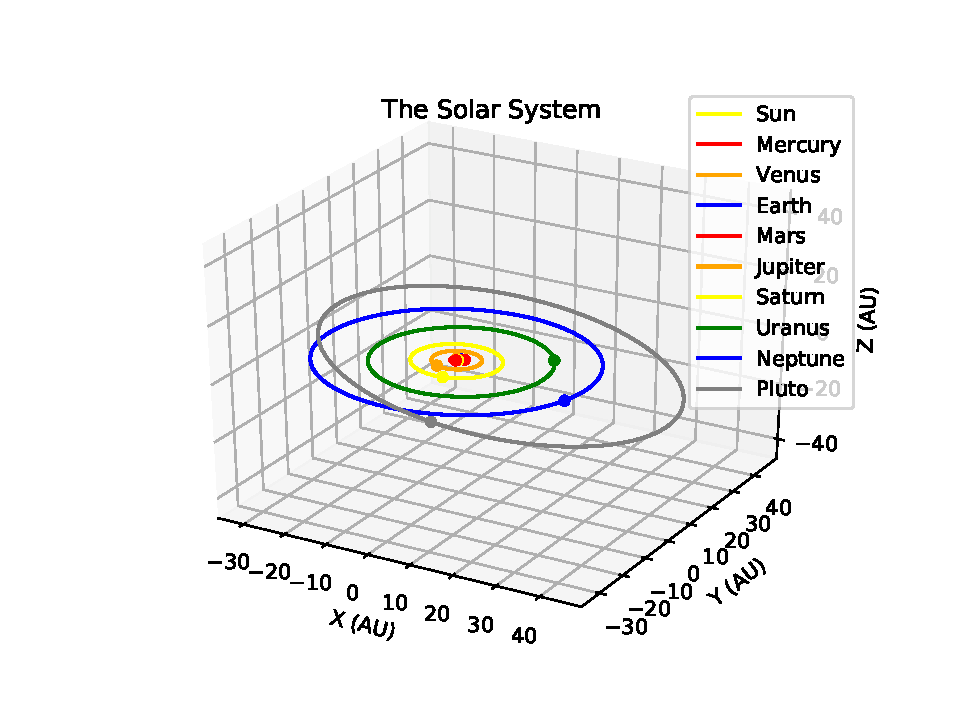
\includegraphics[height=70mm, width=80mm]{Figures/all_planets_isometric.pdf}&
  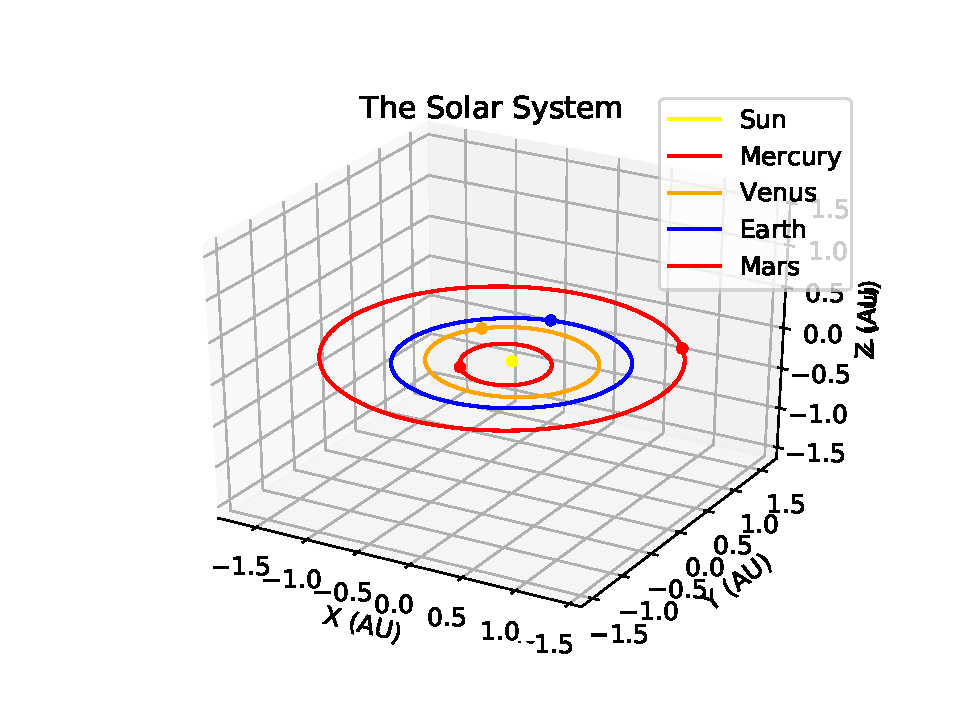
\includegraphics[height=70mm, width=80mm]{Figures/inner_planets_isometric.pdf}\\
  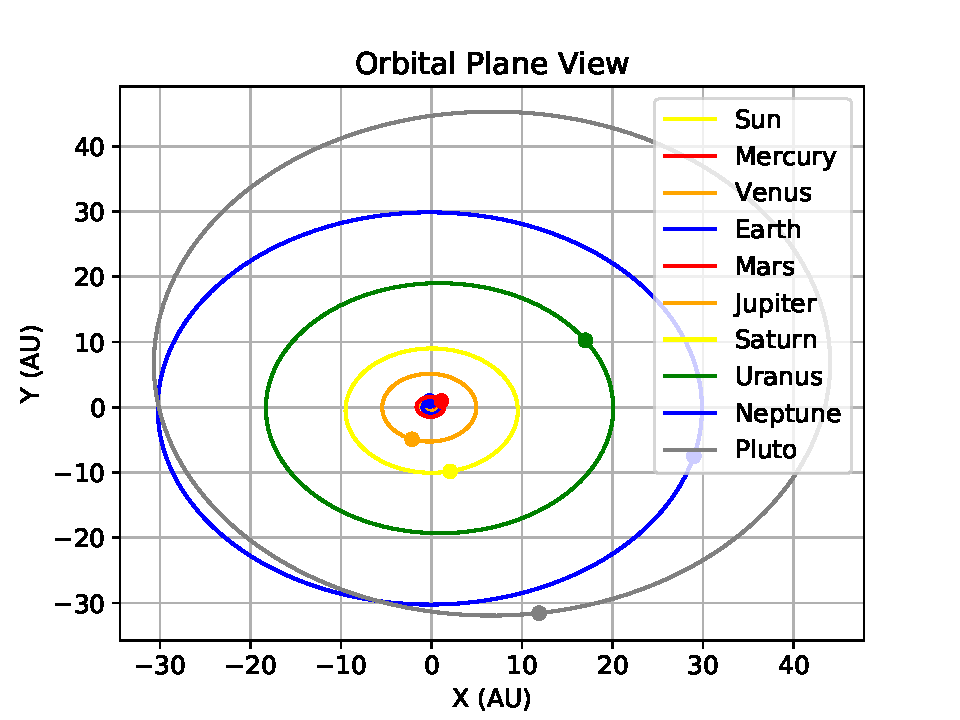
\includegraphics[height=70mm, width=80mm]{Figures/top_down_view_all_planets.pdf}&
  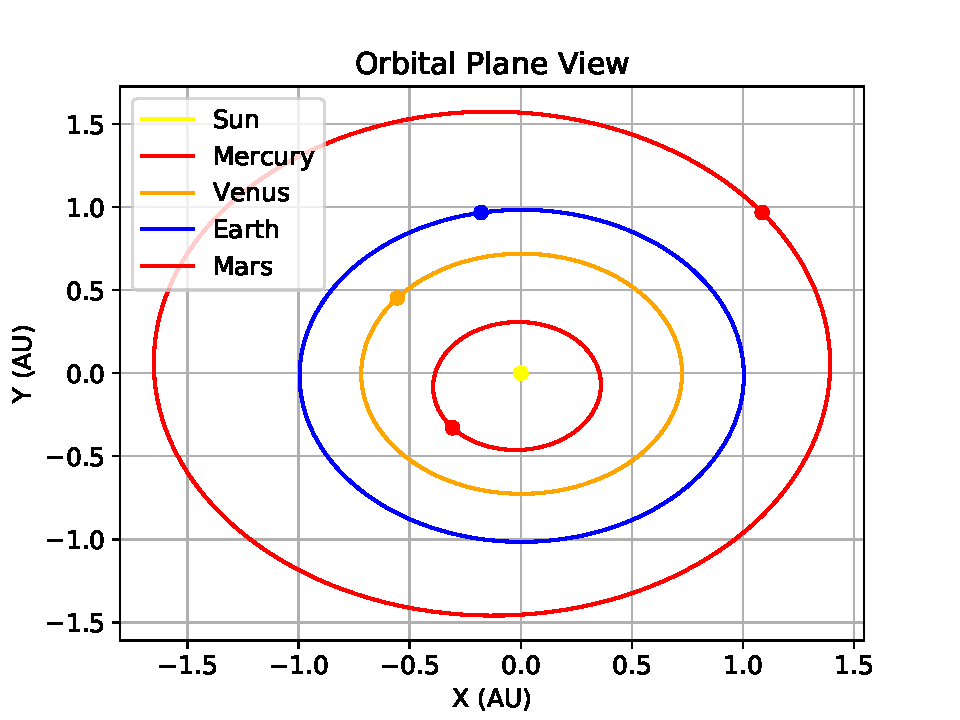
\includegraphics[height=70mm, width=80mm]{Figures/inner_planets_top_down.pdf}\\
  \end{tabular}
  \end{center}
  \caption{Position of Planets using Orbital Elements}
\end{figure}
